% =====================================================================
% vix_product_spec.tex
% Product specification section. Include in main.tex AFTER the
% discussion section with:   % =====================================================================
% vix_product_spec.tex
% Product specification section. Include in main.tex AFTER the
% discussion section with:   % =====================================================================
% vix_product_spec.tex
% Product specification section. Include in main.tex AFTER the
% discussion section with:   % =====================================================================
% vix_product_spec.tex
% Product specification section. Include in main.tex AFTER the
% discussion section with:   \input{vix_product_spec}
%
% Requires in the preamble: amsmath, booktabs, tikz, pgfplots
% (\pgfplotsset{compat=1.16}), and the macros \VIX, \verify, \figplaceholder.
% Uses labels from the discussion section: eq:vix-term, eq:vix-interp, eq:roll.
% New bibliography keys to add: cboewp (already used), cboevxfut, cboevxopt.
% =====================================================================



%=====================================================================
\subsection{Cboe VIX Methodology}
\label{sec:vix-method}
%=====================================================================

The VIX is a model-free estimate of the market's expected 30-day variance, computed from a \emph{strip} of out-of-the-money S\&P~500 (SPX) options. The calculation was introduced in Section~1.1.1: per-expiration variances are given by~\eqref{eq:vix-term} and combined by constant-maturity interpolation in~\eqref{eq:vix-interp}. Here we summarize the rules that determine \emph{which} options enter the calculation, since these rules matter for any implementation.

\paragraph{Options used.} The index uses both standard monthly SPX options (which expire on the third Friday of each month) and weekly SPX options (which expire on other Fridays) \cite{cboewp}. Combining monthly and weekly options ensures that there are always expirations bracketing the 30-day target. Only expirations with 23 to 37 days remaining are eligible: the two maturities immediately surrounding 30 days are designated as the near-term ($T_1$) and next-term ($T_2$) terms. Cboe calculates and disseminates the spot VIX every 15 seconds during trading hours using prevailing market quotes \cite{cboewp}.

\paragraph{Quotes and strike selection.} For each expiration the algorithm proceeds as follows:
\begin{enumerate}
  \item Find the forward level $F$ from put--call parity at the strike where the call and put mid-quotes are closest, and set $K_0$ to the strike at or immediately below $F$ (see Section~1.1.1).
  \item Starting at $K_0$ and moving to \emph{lower} strikes, select out-of-the-money puts. Starting at $K_0$ and moving to \emph{higher} strikes, select out-of-the-money calls. At $K_0$ itself the average of the call and put mid-quotes is used.
  \item Use the mid-quote $Q(K_i)=\tfrac12(\text{bid}+\text{ask})$ for each selected option. Options with a zero bid are never included.
  \item Stop moving outward in a given direction once two consecutive strikes with a zero bid are encountered. No strikes beyond that point are used, even if they have non-zero bids.
\end{enumerate}
The last rule truncates the strip in the far wings, where quotes are stale or non-informative and where a literal evaluation of the formula would be dominated by noise.

\paragraph{Why out-of-the-money options with $1/K^2$ weights.} Each selected option enters~\eqref{eq:vix-term} with weight proportional to $\Delta K_i/K_i^2$. Low-strike puts therefore receive more weight per unit of price than high-strike calls, because they insure against the large downside moves that contribute most to variance. This weighting is exactly the static-replication result for a variance swap, which is derived in the pricing section. Figure~\ref{fig:weights} illustrates the weight function.

\begin{figure}[htbp]
  \centering
  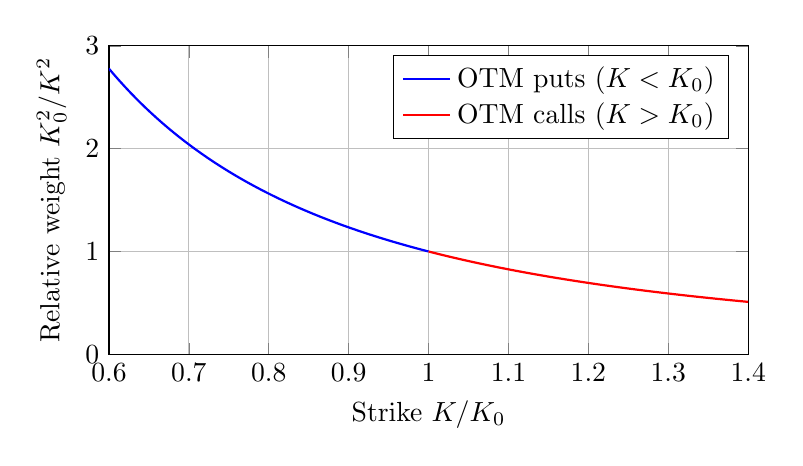
\begin{tikzpicture}
    \begin{axis}[
      width=0.8\linewidth, height=5.5cm,
      xlabel={Strike $K/K_0$}, ylabel={Relative weight $K_0^2/K^2$},
      xmin=0.6, xmax=1.4, ymin=0, ymax=3,
      legend pos=north east, grid=major
    ]
      \addplot[thick, blue, domain=0.6:1, samples=60] {1/x^2};
      \addlegendentry{OTM puts ($K<K_0$)}
      \addplot[thick, red, domain=1:1.4, samples=60] {1/x^2};
      \addlegendentry{OTM calls ($K>K_0$)}
    \end{axis}
  \end{tikzpicture}
  \caption{Variance-swap weight $\propto 1/K^2$ across the option strip (with $\Delta K$ held constant and normalized by $K_0$). Illustrative.}
  \label{fig:weights}
\end{figure}

\paragraph{Spot VIX versus the SOQ.} During trading hours, the spot VIX reflects the average of bid and ask quotes and interpolates between two maturities using~\eqref{eq:vix-interp}. In contrast, expiring VIX futures and options settle for cash against a single official benchmark called the \emph{Special Opening Quotation} (SOQ) \cite{cboewp}. The SOQ differs from the spot VIX in two important ways:
\begin{enumerate}
  \item \textbf{Single 30-day expiration.} Because settlement occurs on a Wednesday morning exactly 30 days before the underlying SPX options expire, the SOQ evaluates the forward variance formula~\eqref{eq:vix-term} on that single expiration. No two-maturity interpolation~\eqref{eq:vix-interp} is needed.
  \item \textbf{Actual opening trade prices.} Rather than midpoint quotes, the SOQ uses actual executed prices from a special opening auction on settlement morning (falling back to mid-quotes only if an option does not trade).
\end{enumerate}
Because of these structural differences, the settlement SOQ can diverge from the spot VIX displayed on screens that morning.

%=====================================================================
\subsection{VIX Futures}
\label{sec:vix-futures}
%=====================================================================

A VIX future is a cash-settled contract whose final value is the VIX SOQ on the expiration date \cite{cboevxfut}. The contract is not on the VIX ``spot'' that traders see during the day, nor on a basket of SPX options held by the exchange; it is a standardized bet on the SOQ.

\paragraph{Key contract terms.}
\begin{table}[htbp]
\centering
\small
\begin{tabular}{@{}p{3.6cm}p{11cm}@{}}
\toprule
\textbf{Term} & \textbf{Specification}\\
\midrule
Underlying & Cboe Volatility Index (settled at the SOQ)\\
Multiplier & \$1{,}000 per index point\\
Settlement & Cash, at the SOQ on the final settlement date\\
Final settlement date & Wednesday that is 30 days before the third Friday of the following calendar month (previous business day if a holiday)\verify\\
Expirations & Several consecutive monthly expirations, plus weekly series\verify\\
\bottomrule
\end{tabular}
\caption{Principal terms of standard VIX futures. Check the exchange contract specification before finalizing.}
\label{tab:vx-spec}
\end{table}

The settlement date is chosen so that the 30-day window of the SPX options used to compute the SOQ begins at the futures expiration. The futures are therefore a view on volatility over the \emph{next} 30 days \emph{starting at expiry}, not over the life of the contract.

\paragraph{Payoff.} Entering a long position at futures price $F_0$ and holding until expiration $T$ produces the profit
\begin{equation}
  \text{P\&L} = 1{,}000\times(\text{SOQ}_T - F_0),
\end{equation}
before margin and financing considerations. For example, buying at $F_0=18.50$ and settling at $\text{SOQ}_T = 21.30$ gives $1{,}000\times 2.80=\$2{,}800$ per contract (hypothetical numbers).

\paragraph{Futures versus spot VIX.} Before expiry the futures price is not equal to the spot VIX. Under the risk-neutral measure $\mathbb{Q}$,
\begin{equation}
  F(t,T) = \mathbb{E}^{\mathbb{Q}}\!\left[\text{SOQ}_T \,\middle|\, \mathcal{F}_t\right],
  \label{eq:fut-expect}
\end{equation}
so the futures price is the expected \emph{future} level of the index. It differs from the spot VIX because (i) the market expects mean reversion in volatility, (ii) the VIX is the square root of a variance, introducing a convexity effect (Jensen's inequality), and (iii) hedgers pay a premium for volatility protection. The convexity effect is quantified in the pricing and simulation sections.

\paragraph{Smaller contracts.} Cboe also lists mini VIX futures with a smaller multiplier (\$100 per point)\verify, useful for smaller accounts and hedges.

%=====================================================================
\subsection{VIX Options}
\label{sec:vix-options}
%=====================================================================

VIX options are European-style, cash-settled options on the VIX with a multiplier of \$100 per index point \cite{cboevxopt}. They settle to the same SOQ as the futures with the matching expiration.

\begin{table}[htbp]
\centering
\small
\begin{tabular}{@{}p{3.6cm}p{11cm}@{}}
\toprule
\textbf{Term} & \textbf{Specification}\\
\midrule
Underlying & VIX (settled at the SOQ); priced off the VIX future with the same expiration\\
Style & European\\
Multiplier & \$100 per index point\\
Settlement & Cash, at the SOQ on the expiration date\\
Expirations & Same schedule as VIX futures (monthly, with weekly series)\verify\\
\bottomrule
\end{tabular}
\caption{Principal terms of VIX options.}
\label{tab:vix-options}
\end{table}

\paragraph{Payoff.} At expiration a call with strike $K$ pays $100\times\max(\text{SOQ}_T-K,\,0)$ and a put pays $100\times\max(K-\text{SOQ}_T,\,0)$. For instance, a call with $K=20$ settling at $\text{SOQ}_T=23.50$ pays $100\times 3.50 = \$350$ (hypothetical).

\paragraph{The underlying is the future, not spot.} Because the VIX itself is not tradable, VIX options cannot be hedged with the spot index. Their effective underlying is the VIX future with the same expiration, which \emph{can} be traded. Consequently put--call parity takes the form
\begin{equation}
  C(K,T) - P(K,T) = e^{-r(T-t)}\big(F(t,T)-K\big),
  \label{eq:vix-pcp}
\end{equation}
where $F(t,T)$ is the VIX future for the same expiration, \emph{not} the spot VIX. Pricing VIX options therefore requires a model of the dynamics of $F(t,T)$, usually a stochastic-volatility model; this is the role of the Heston simulation later in this report.

%=====================================================================
\subsection{The Term Structure of VIX Futures}
\label{sec:term-structure}
%=====================================================================

At each date $t$ there is a family of listed VIX futures with different expirations. The map $T\mapsto F(t,T)$ is the \emph{term structure} (or \emph{forward curve}) of volatility.

\begin{itemize}
  \item \textbf{Contango:} the curve slopes upward, $F(t,T_1) < F(t,T_2) < \cdots$, with the front future typically above the spot VIX. This is the usual shape in calm markets.
  \item \textbf{Backwardation:} the curve slopes downward, $F(t,T_1) > F(t,T_2) > \cdots$, with the spot VIX at or above the front future. This typically occurs during market stress, when the spot VIX spikes.
\end{itemize}

\paragraph{Why the curve has these shapes.} The VIX is mean-reverting: it tends to return toward a long-run level $\theta$. A stylized representation, ignoring convexity and risk premia, is
\begin{equation}
  F(t,T) \approx \theta + (S_t-\theta)\,e^{-\kappa(T-t)},
  \label{eq:stylized-curve}
\end{equation}
where $S_t$ is the current spot VIX and $\kappa>0$ is the speed of mean reversion. When $S_t<\theta$ (calm markets) the curve rises toward $\theta$ (contango); when $S_t>\theta$ (stressed markets) it falls toward $\theta$ (backwardation). Figure~\ref{fig:term-structure} illustrates both cases schematically, and Figure~\ref{fig:term-structure-real} displays the actual observed term structures during the February 2018 Volmageddon and March 2020 COVID-19 episodes. In practice, a risk premium paid by hedgers also pushes the curve upward, which is one reason contango is more common than backwardation\verify.

\begin{figure}[htbp]
  \centering
  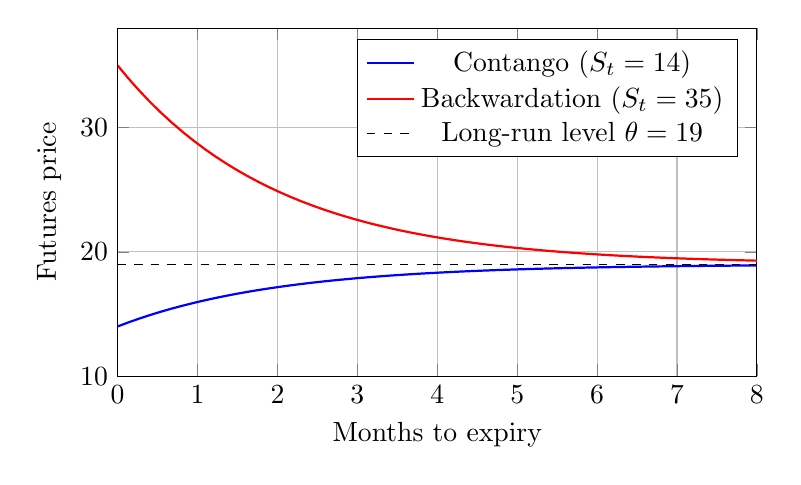
\begin{tikzpicture}
    \begin{axis}[
      width=0.8\linewidth, height=6cm,
      xlabel={Months to expiry}, ylabel={Futures price},
      xmin=0, xmax=8, ymin=10, ymax=38,
      legend pos=north east, grid=major
    ]
      \addplot[thick, blue, domain=0:8, samples=60] {19 + (14-19)*exp(-0.5*x)};
      \addlegendentry{Contango ($S_t=14$)}
      \addplot[thick, red, domain=0:8, samples=60] {19 + (35-19)*exp(-0.5*x)};
      \addlegendentry{Backwardation ($S_t=35$)}
      \addplot[dashed, black, domain=0:8] {19};
      \addlegendentry{Long-run level $\theta=19$}
    \end{axis}
  \end{tikzpicture}
  \caption{Stylized VIX futures curves from~\eqref{eq:stylized-curve} with assumed $\theta=19$ and $\kappa=0.5$ per month. Illustrative only, not market data.}
  \label{fig:term-structure}
\end{figure}

\begin{figure}[htbp]
  \centering
  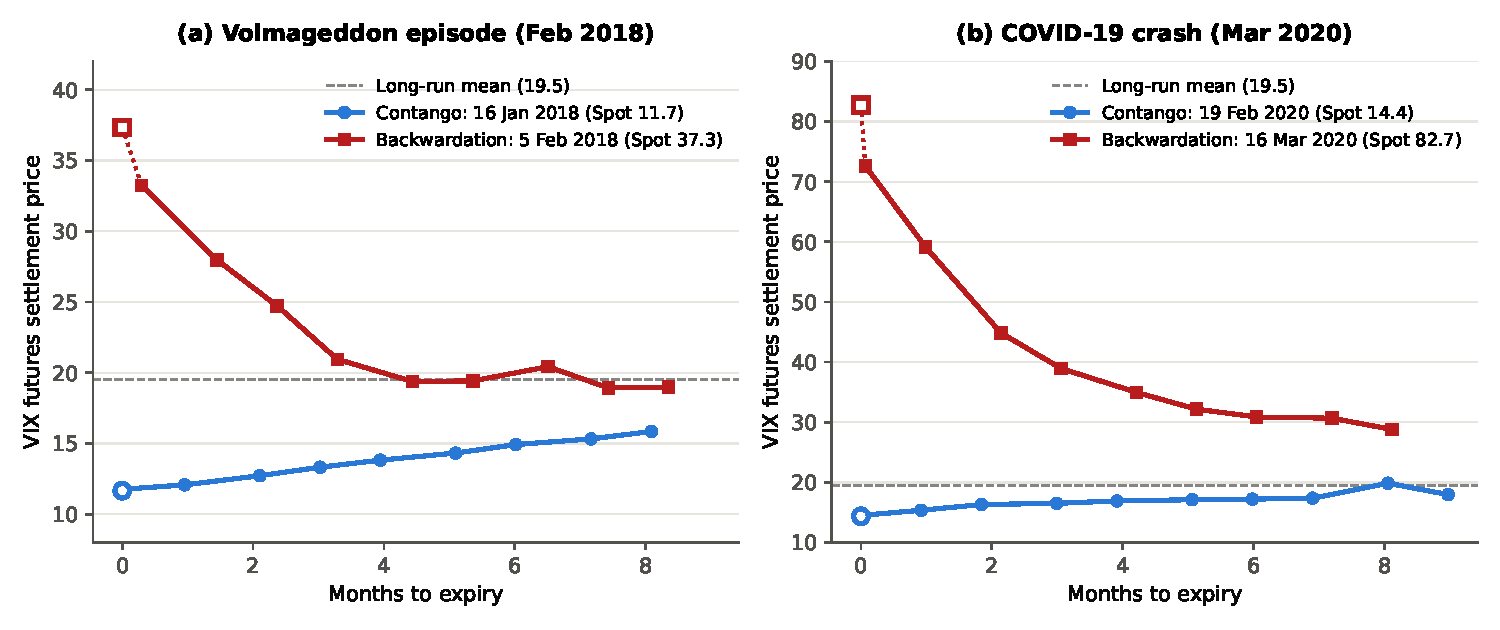
\includegraphics[width=\linewidth]{figures/vix_term_structure.pdf}
  \caption{Observed VIX futures term structure during calm and stressed markets: (a) the February 2018 Volmageddon episode (16 January vs.\ 5 February 2018) and (b) the COVID-19 market crash (19 February vs.\ 16 March 2020). Hollow markers at month 0 denote the prevailing spot VIX; solid markers denote official Cboe futures settlement prices. The dashed line marks the empirical long-run mean ($\approx 19.5$). Data: Cboe Futures Exchange and Cboe.}
  \label{fig:term-structure-real}
\end{figure}

\paragraph{Consequences for investors.} The shape of the curve determines the carry of a long or short volatility position. Summarizing the roll discussion in the previous section (see~\eqref{eq:roll}):

\begin{table}[htbp]
\centering
\small
\begin{tabular}{@{}lccc@{}}
\toprule
\textbf{Curve shape} & \textbf{Typical state} & \textbf{Long futures (roll)} & \textbf{Short futures (roll)}\\
\midrule
Contango & Calm market & Negative roll yield & Positive roll yield\\
Backwardation & Market stress & Positive roll yield & Negative roll yield\\
\bottomrule
\end{tabular}
\caption{Effect of term-structure shape on the carry of VIX futures positions, assuming an unchanged spot VIX.}
\label{tab:roll-summary}
\end{table}

A common summary of the slope is the \emph{basis} $F(t,T_1)-\text{VIX}_t$ or the relative spread $\big(F(t,T_2)-F(t,T_1)\big)/F(t,T_1)$ between the first two futures. These quantities will be used in the backtest to explain when a long-futures hedge is expensive to hold.
%
% Requires in the preamble: amsmath, booktabs, tikz, pgfplots
% (\pgfplotsset{compat=1.16}), and the macros \VIX, \verify, \figplaceholder.
% Uses labels from the discussion section: eq:vix-term, eq:vix-interp, eq:roll.
% New bibliography keys to add: cboewp (already used), cboevxfut, cboevxopt.
% =====================================================================



%=====================================================================
\subsection{Cboe VIX Methodology}
\label{sec:vix-method}
%=====================================================================

The VIX is a model-free estimate of the market's expected 30-day variance, computed from a \emph{strip} of out-of-the-money S\&P~500 (SPX) options. The calculation was introduced in Section~1.1.1: per-expiration variances are given by~\eqref{eq:vix-term} and combined by constant-maturity interpolation in~\eqref{eq:vix-interp}. Here we summarize the rules that determine \emph{which} options enter the calculation, since these rules matter for any implementation.

\paragraph{Options used.} The index uses both standard monthly SPX options (which expire on the third Friday of each month) and weekly SPX options (which expire on other Fridays) \cite{cboewp}. Combining monthly and weekly options ensures that there are always expirations bracketing the 30-day target. Only expirations with 23 to 37 days remaining are eligible: the two maturities immediately surrounding 30 days are designated as the near-term ($T_1$) and next-term ($T_2$) terms. Cboe calculates and disseminates the spot VIX every 15 seconds during trading hours using prevailing market quotes \cite{cboewp}.

\paragraph{Quotes and strike selection.} For each expiration the algorithm proceeds as follows:
\begin{enumerate}
  \item Find the forward level $F$ from put--call parity at the strike where the call and put mid-quotes are closest, and set $K_0$ to the strike at or immediately below $F$ (see Section~1.1.1).
  \item Starting at $K_0$ and moving to \emph{lower} strikes, select out-of-the-money puts. Starting at $K_0$ and moving to \emph{higher} strikes, select out-of-the-money calls. At $K_0$ itself the average of the call and put mid-quotes is used.
  \item Use the mid-quote $Q(K_i)=\tfrac12(\text{bid}+\text{ask})$ for each selected option. Options with a zero bid are never included.
  \item Stop moving outward in a given direction once two consecutive strikes with a zero bid are encountered. No strikes beyond that point are used, even if they have non-zero bids.
\end{enumerate}
The last rule truncates the strip in the far wings, where quotes are stale or non-informative and where a literal evaluation of the formula would be dominated by noise.

\paragraph{Why out-of-the-money options with $1/K^2$ weights.} Each selected option enters~\eqref{eq:vix-term} with weight proportional to $\Delta K_i/K_i^2$. Low-strike puts therefore receive more weight per unit of price than high-strike calls, because they insure against the large downside moves that contribute most to variance. This weighting is exactly the static-replication result for a variance swap, which is derived in the pricing section. Figure~\ref{fig:weights} illustrates the weight function.

\begin{figure}[htbp]
  \centering
  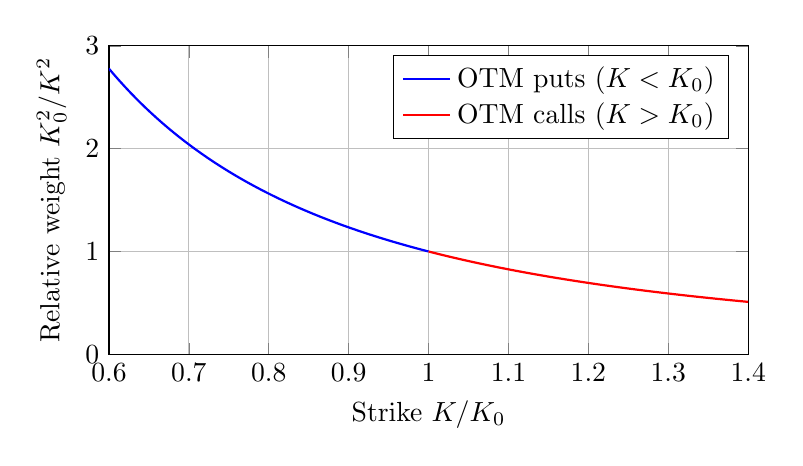
\begin{tikzpicture}
    \begin{axis}[
      width=0.8\linewidth, height=5.5cm,
      xlabel={Strike $K/K_0$}, ylabel={Relative weight $K_0^2/K^2$},
      xmin=0.6, xmax=1.4, ymin=0, ymax=3,
      legend pos=north east, grid=major
    ]
      \addplot[thick, blue, domain=0.6:1, samples=60] {1/x^2};
      \addlegendentry{OTM puts ($K<K_0$)}
      \addplot[thick, red, domain=1:1.4, samples=60] {1/x^2};
      \addlegendentry{OTM calls ($K>K_0$)}
    \end{axis}
  \end{tikzpicture}
  \caption{Variance-swap weight $\propto 1/K^2$ across the option strip (with $\Delta K$ held constant and normalized by $K_0$). Illustrative.}
  \label{fig:weights}
\end{figure}

\paragraph{Spot VIX versus the SOQ.} During trading hours, the spot VIX reflects the average of bid and ask quotes and interpolates between two maturities using~\eqref{eq:vix-interp}. In contrast, expiring VIX futures and options settle for cash against a single official benchmark called the \emph{Special Opening Quotation} (SOQ) \cite{cboewp}. The SOQ differs from the spot VIX in two important ways:
\begin{enumerate}
  \item \textbf{Single 30-day expiration.} Because settlement occurs on a Wednesday morning exactly 30 days before the underlying SPX options expire, the SOQ evaluates the forward variance formula~\eqref{eq:vix-term} on that single expiration. No two-maturity interpolation~\eqref{eq:vix-interp} is needed.
  \item \textbf{Actual opening trade prices.} Rather than midpoint quotes, the SOQ uses actual executed prices from a special opening auction on settlement morning (falling back to mid-quotes only if an option does not trade).
\end{enumerate}
Because of these structural differences, the settlement SOQ can diverge from the spot VIX displayed on screens that morning.

%=====================================================================
\subsection{VIX Futures}
\label{sec:vix-futures}
%=====================================================================

A VIX future is a cash-settled contract whose final value is the VIX SOQ on the expiration date \cite{cboevxfut}. The contract is not on the VIX ``spot'' that traders see during the day, nor on a basket of SPX options held by the exchange; it is a standardized bet on the SOQ.

\paragraph{Key contract terms.}
\begin{table}[htbp]
\centering
\small
\begin{tabular}{@{}p{3.6cm}p{11cm}@{}}
\toprule
\textbf{Term} & \textbf{Specification}\\
\midrule
Underlying & Cboe Volatility Index (settled at the SOQ)\\
Multiplier & \$1{,}000 per index point\\
Settlement & Cash, at the SOQ on the final settlement date\\
Final settlement date & Wednesday that is 30 days before the third Friday of the following calendar month (previous business day if a holiday)\verify\\
Expirations & Several consecutive monthly expirations, plus weekly series\verify\\
\bottomrule
\end{tabular}
\caption{Principal terms of standard VIX futures. Check the exchange contract specification before finalizing.}
\label{tab:vx-spec}
\end{table}

The settlement date is chosen so that the 30-day window of the SPX options used to compute the SOQ begins at the futures expiration. The futures are therefore a view on volatility over the \emph{next} 30 days \emph{starting at expiry}, not over the life of the contract.

\paragraph{Payoff.} Entering a long position at futures price $F_0$ and holding until expiration $T$ produces the profit
\begin{equation}
  \text{P\&L} = 1{,}000\times(\text{SOQ}_T - F_0),
\end{equation}
before margin and financing considerations. For example, buying at $F_0=18.50$ and settling at $\text{SOQ}_T = 21.30$ gives $1{,}000\times 2.80=\$2{,}800$ per contract (hypothetical numbers).

\paragraph{Futures versus spot VIX.} Before expiry the futures price is not equal to the spot VIX. Under the risk-neutral measure $\mathbb{Q}$,
\begin{equation}
  F(t,T) = \mathbb{E}^{\mathbb{Q}}\!\left[\text{SOQ}_T \,\middle|\, \mathcal{F}_t\right],
  \label{eq:fut-expect}
\end{equation}
so the futures price is the expected \emph{future} level of the index. It differs from the spot VIX because (i) the market expects mean reversion in volatility, (ii) the VIX is the square root of a variance, introducing a convexity effect (Jensen's inequality), and (iii) hedgers pay a premium for volatility protection. The convexity effect is quantified in the pricing and simulation sections.

\paragraph{Smaller contracts.} Cboe also lists mini VIX futures with a smaller multiplier (\$100 per point)\verify, useful for smaller accounts and hedges.

%=====================================================================
\subsection{VIX Options}
\label{sec:vix-options}
%=====================================================================

VIX options are European-style, cash-settled options on the VIX with a multiplier of \$100 per index point \cite{cboevxopt}. They settle to the same SOQ as the futures with the matching expiration.

\begin{table}[htbp]
\centering
\small
\begin{tabular}{@{}p{3.6cm}p{11cm}@{}}
\toprule
\textbf{Term} & \textbf{Specification}\\
\midrule
Underlying & VIX (settled at the SOQ); priced off the VIX future with the same expiration\\
Style & European\\
Multiplier & \$100 per index point\\
Settlement & Cash, at the SOQ on the expiration date\\
Expirations & Same schedule as VIX futures (monthly, with weekly series)\verify\\
\bottomrule
\end{tabular}
\caption{Principal terms of VIX options.}
\label{tab:vix-options}
\end{table}

\paragraph{Payoff.} At expiration a call with strike $K$ pays $100\times\max(\text{SOQ}_T-K,\,0)$ and a put pays $100\times\max(K-\text{SOQ}_T,\,0)$. For instance, a call with $K=20$ settling at $\text{SOQ}_T=23.50$ pays $100\times 3.50 = \$350$ (hypothetical).

\paragraph{The underlying is the future, not spot.} Because the VIX itself is not tradable, VIX options cannot be hedged with the spot index. Their effective underlying is the VIX future with the same expiration, which \emph{can} be traded. Consequently put--call parity takes the form
\begin{equation}
  C(K,T) - P(K,T) = e^{-r(T-t)}\big(F(t,T)-K\big),
  \label{eq:vix-pcp}
\end{equation}
where $F(t,T)$ is the VIX future for the same expiration, \emph{not} the spot VIX. Pricing VIX options therefore requires a model of the dynamics of $F(t,T)$, usually a stochastic-volatility model; this is the role of the Heston simulation later in this report.

%=====================================================================
\subsection{The Term Structure of VIX Futures}
\label{sec:term-structure}
%=====================================================================

At each date $t$ there is a family of listed VIX futures with different expirations. The map $T\mapsto F(t,T)$ is the \emph{term structure} (or \emph{forward curve}) of volatility.

\begin{itemize}
  \item \textbf{Contango:} the curve slopes upward, $F(t,T_1) < F(t,T_2) < \cdots$, with the front future typically above the spot VIX. This is the usual shape in calm markets.
  \item \textbf{Backwardation:} the curve slopes downward, $F(t,T_1) > F(t,T_2) > \cdots$, with the spot VIX at or above the front future. This typically occurs during market stress, when the spot VIX spikes.
\end{itemize}

\paragraph{Why the curve has these shapes.} The VIX is mean-reverting: it tends to return toward a long-run level $\theta$. A stylized representation, ignoring convexity and risk premia, is
\begin{equation}
  F(t,T) \approx \theta + (S_t-\theta)\,e^{-\kappa(T-t)},
  \label{eq:stylized-curve}
\end{equation}
where $S_t$ is the current spot VIX and $\kappa>0$ is the speed of mean reversion. When $S_t<\theta$ (calm markets) the curve rises toward $\theta$ (contango); when $S_t>\theta$ (stressed markets) it falls toward $\theta$ (backwardation). Figure~\ref{fig:term-structure} illustrates both cases schematically, and Figure~\ref{fig:term-structure-real} displays the actual observed term structures during the February 2018 Volmageddon and March 2020 COVID-19 episodes. In practice, a risk premium paid by hedgers also pushes the curve upward, which is one reason contango is more common than backwardation\verify.

\begin{figure}[htbp]
  \centering
  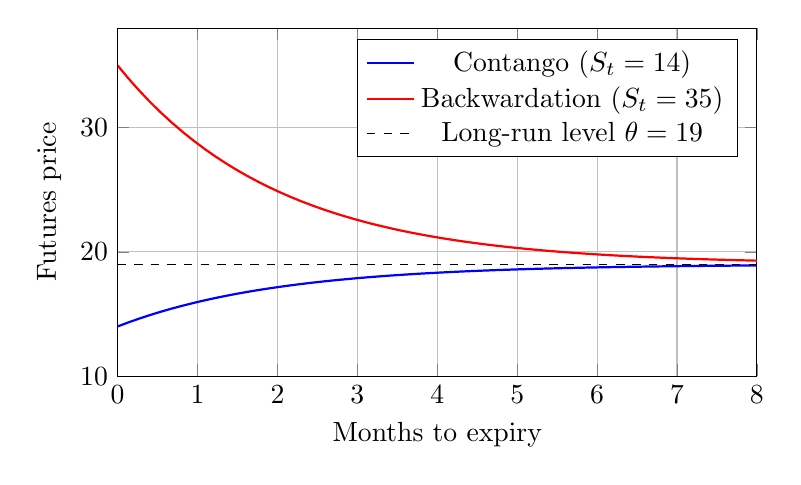
\begin{tikzpicture}
    \begin{axis}[
      width=0.8\linewidth, height=6cm,
      xlabel={Months to expiry}, ylabel={Futures price},
      xmin=0, xmax=8, ymin=10, ymax=38,
      legend pos=north east, grid=major
    ]
      \addplot[thick, blue, domain=0:8, samples=60] {19 + (14-19)*exp(-0.5*x)};
      \addlegendentry{Contango ($S_t=14$)}
      \addplot[thick, red, domain=0:8, samples=60] {19 + (35-19)*exp(-0.5*x)};
      \addlegendentry{Backwardation ($S_t=35$)}
      \addplot[dashed, black, domain=0:8] {19};
      \addlegendentry{Long-run level $\theta=19$}
    \end{axis}
  \end{tikzpicture}
  \caption{Stylized VIX futures curves from~\eqref{eq:stylized-curve} with assumed $\theta=19$ and $\kappa=0.5$ per month. Illustrative only, not market data.}
  \label{fig:term-structure}
\end{figure}

\begin{figure}[htbp]
  \centering
  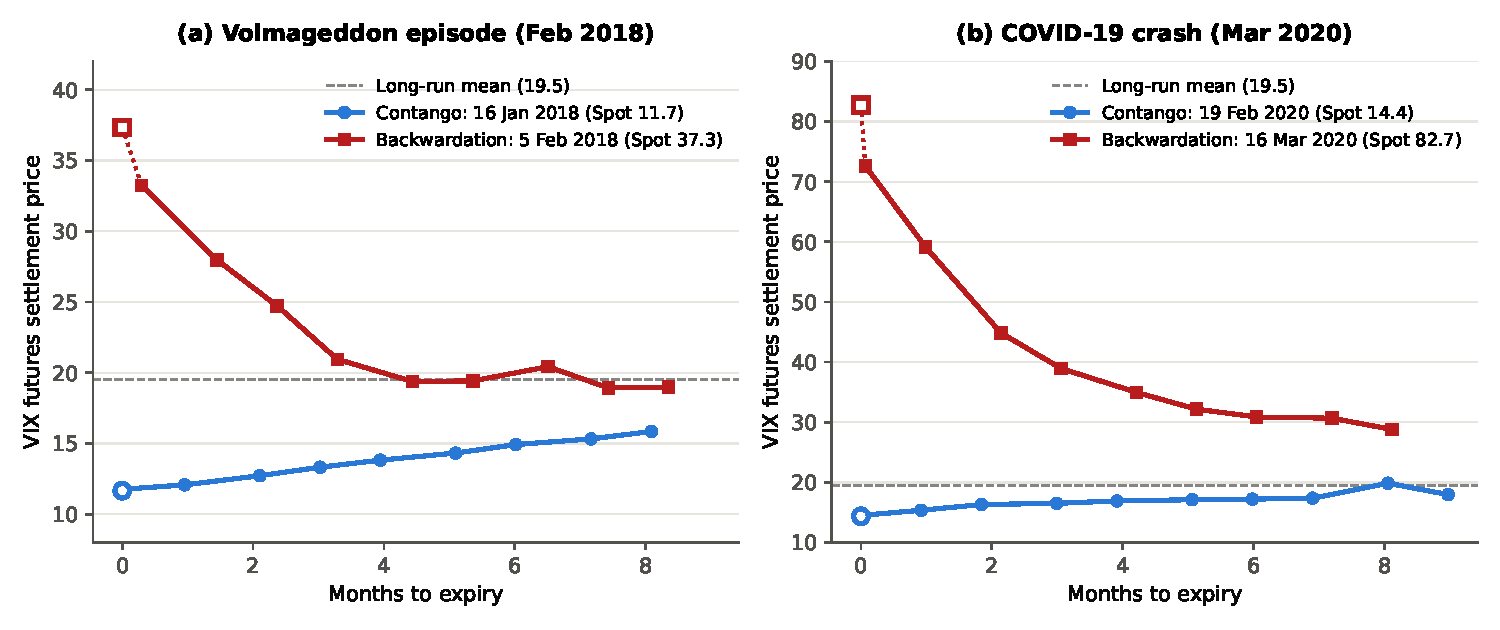
\includegraphics[width=\linewidth]{figures/vix_term_structure.pdf}
  \caption{Observed VIX futures term structure during calm and stressed markets: (a) the February 2018 Volmageddon episode (16 January vs.\ 5 February 2018) and (b) the COVID-19 market crash (19 February vs.\ 16 March 2020). Hollow markers at month 0 denote the prevailing spot VIX; solid markers denote official Cboe futures settlement prices. The dashed line marks the empirical long-run mean ($\approx 19.5$). Data: Cboe Futures Exchange and Cboe.}
  \label{fig:term-structure-real}
\end{figure}

\paragraph{Consequences for investors.} The shape of the curve determines the carry of a long or short volatility position. Summarizing the roll discussion in the previous section (see~\eqref{eq:roll}):

\begin{table}[htbp]
\centering
\small
\begin{tabular}{@{}lccc@{}}
\toprule
\textbf{Curve shape} & \textbf{Typical state} & \textbf{Long futures (roll)} & \textbf{Short futures (roll)}\\
\midrule
Contango & Calm market & Negative roll yield & Positive roll yield\\
Backwardation & Market stress & Positive roll yield & Negative roll yield\\
\bottomrule
\end{tabular}
\caption{Effect of term-structure shape on the carry of VIX futures positions, assuming an unchanged spot VIX.}
\label{tab:roll-summary}
\end{table}

A common summary of the slope is the \emph{basis} $F(t,T_1)-\text{VIX}_t$ or the relative spread $\big(F(t,T_2)-F(t,T_1)\big)/F(t,T_1)$ between the first two futures. These quantities will be used in the backtest to explain when a long-futures hedge is expensive to hold.
%
% Requires in the preamble: amsmath, booktabs, tikz, pgfplots
% (\pgfplotsset{compat=1.16}), and the macros \VIX, \verify, \figplaceholder.
% Uses labels from the discussion section: eq:vix-term, eq:vix-interp, eq:roll.
% New bibliography keys to add: cboewp (already used), cboevxfut, cboevxopt.
% =====================================================================



%=====================================================================
\subsection{Cboe VIX Methodology}
\label{sec:vix-method}
%=====================================================================

The VIX is a model-free estimate of the market's expected 30-day variance, computed from a \emph{strip} of out-of-the-money S\&P~500 (SPX) options. The calculation was introduced in Section~1.1.1: per-expiration variances are given by~\eqref{eq:vix-term} and combined by constant-maturity interpolation in~\eqref{eq:vix-interp}. Here we summarize the rules that determine \emph{which} options enter the calculation, since these rules matter for any implementation.

\paragraph{Options used.} The index uses both standard monthly SPX options (which expire on the third Friday of each month) and weekly SPX options (which expire on other Fridays) \cite{cboewp}. Combining monthly and weekly options ensures that there are always expirations bracketing the 30-day target. Only expirations with 23 to 37 days remaining are eligible: the two maturities immediately surrounding 30 days are designated as the near-term ($T_1$) and next-term ($T_2$) terms. Cboe calculates and disseminates the spot VIX every 15 seconds during trading hours using prevailing market quotes \cite{cboewp}.

\paragraph{Quotes and strike selection.} For each expiration the algorithm proceeds as follows:
\begin{enumerate}
  \item Find the forward level $F$ from put--call parity at the strike where the call and put mid-quotes are closest, and set $K_0$ to the strike at or immediately below $F$ (see Section~1.1.1).
  \item Starting at $K_0$ and moving to \emph{lower} strikes, select out-of-the-money puts. Starting at $K_0$ and moving to \emph{higher} strikes, select out-of-the-money calls. At $K_0$ itself the average of the call and put mid-quotes is used.
  \item Use the mid-quote $Q(K_i)=\tfrac12(\text{bid}+\text{ask})$ for each selected option. Options with a zero bid are never included.
  \item Stop moving outward in a given direction once two consecutive strikes with a zero bid are encountered. No strikes beyond that point are used, even if they have non-zero bids.
\end{enumerate}
The last rule truncates the strip in the far wings, where quotes are stale or non-informative and where a literal evaluation of the formula would be dominated by noise.

\paragraph{Why out-of-the-money options with $1/K^2$ weights.} Each selected option enters~\eqref{eq:vix-term} with weight proportional to $\Delta K_i/K_i^2$. Low-strike puts therefore receive more weight per unit of price than high-strike calls, because they insure against the large downside moves that contribute most to variance. This weighting is exactly the static-replication result for a variance swap, which is derived in the pricing section. Figure~\ref{fig:weights} illustrates the weight function.

\begin{figure}[htbp]
  \centering
  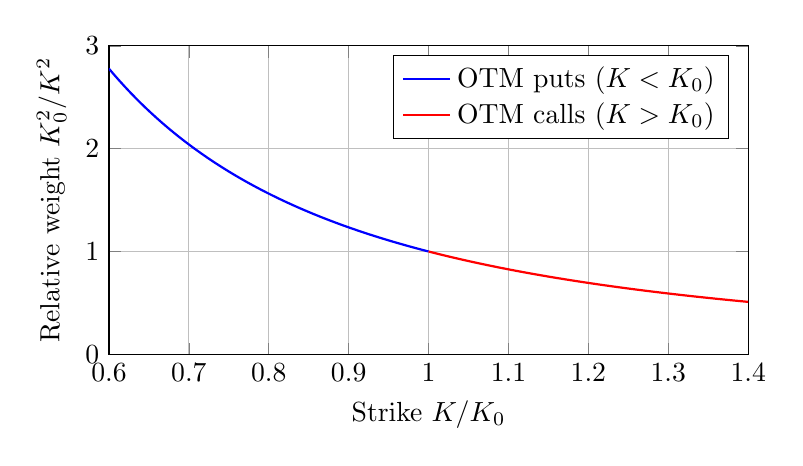
\begin{tikzpicture}
    \begin{axis}[
      width=0.8\linewidth, height=5.5cm,
      xlabel={Strike $K/K_0$}, ylabel={Relative weight $K_0^2/K^2$},
      xmin=0.6, xmax=1.4, ymin=0, ymax=3,
      legend pos=north east, grid=major
    ]
      \addplot[thick, blue, domain=0.6:1, samples=60] {1/x^2};
      \addlegendentry{OTM puts ($K<K_0$)}
      \addplot[thick, red, domain=1:1.4, samples=60] {1/x^2};
      \addlegendentry{OTM calls ($K>K_0$)}
    \end{axis}
  \end{tikzpicture}
  \caption{Variance-swap weight $\propto 1/K^2$ across the option strip (with $\Delta K$ held constant and normalized by $K_0$). Illustrative.}
  \label{fig:weights}
\end{figure}

\paragraph{Spot VIX versus the SOQ.} During trading hours, the spot VIX reflects the average of bid and ask quotes and interpolates between two maturities using~\eqref{eq:vix-interp}. In contrast, expiring VIX futures and options settle for cash against a single official benchmark called the \emph{Special Opening Quotation} (SOQ) \cite{cboewp}. The SOQ differs from the spot VIX in two important ways:
\begin{enumerate}
  \item \textbf{Single 30-day expiration.} Because settlement occurs on a Wednesday morning exactly 30 days before the underlying SPX options expire, the SOQ evaluates the forward variance formula~\eqref{eq:vix-term} on that single expiration. No two-maturity interpolation~\eqref{eq:vix-interp} is needed.
  \item \textbf{Actual opening trade prices.} Rather than midpoint quotes, the SOQ uses actual executed prices from a special opening auction on settlement morning (falling back to mid-quotes only if an option does not trade).
\end{enumerate}
Because of these structural differences, the settlement SOQ can diverge from the spot VIX displayed on screens that morning.

%=====================================================================
\subsection{VIX Futures}
\label{sec:vix-futures}
%=====================================================================

A VIX future is a cash-settled contract whose final value is the VIX SOQ on the expiration date \cite{cboevxfut}. The contract is not on the VIX ``spot'' that traders see during the day, nor on a basket of SPX options held by the exchange; it is a standardized bet on the SOQ.

\paragraph{Key contract terms.}
\begin{table}[htbp]
\centering
\small
\begin{tabular}{@{}p{3.6cm}p{11cm}@{}}
\toprule
\textbf{Term} & \textbf{Specification}\\
\midrule
Underlying & Cboe Volatility Index (settled at the SOQ)\\
Multiplier & \$1{,}000 per index point\\
Settlement & Cash, at the SOQ on the final settlement date\\
Final settlement date & Wednesday that is 30 days before the third Friday of the following calendar month (previous business day if a holiday)\verify\\
Expirations & Several consecutive monthly expirations, plus weekly series\verify\\
\bottomrule
\end{tabular}
\caption{Principal terms of standard VIX futures. Check the exchange contract specification before finalizing.}
\label{tab:vx-spec}
\end{table}

The settlement date is chosen so that the 30-day window of the SPX options used to compute the SOQ begins at the futures expiration. The futures are therefore a view on volatility over the \emph{next} 30 days \emph{starting at expiry}, not over the life of the contract.

\paragraph{Payoff.} Entering a long position at futures price $F_0$ and holding until expiration $T$ produces the profit
\begin{equation}
  \text{P\&L} = 1{,}000\times(\text{SOQ}_T - F_0),
\end{equation}
before margin and financing considerations. For example, buying at $F_0=18.50$ and settling at $\text{SOQ}_T = 21.30$ gives $1{,}000\times 2.80=\$2{,}800$ per contract (hypothetical numbers).

\paragraph{Futures versus spot VIX.} Before expiry the futures price is not equal to the spot VIX. Under the risk-neutral measure $\mathbb{Q}$,
\begin{equation}
  F(t,T) = \mathbb{E}^{\mathbb{Q}}\!\left[\text{SOQ}_T \,\middle|\, \mathcal{F}_t\right],
  \label{eq:fut-expect}
\end{equation}
so the futures price is the expected \emph{future} level of the index. It differs from the spot VIX because (i) the market expects mean reversion in volatility, (ii) the VIX is the square root of a variance, introducing a convexity effect (Jensen's inequality), and (iii) hedgers pay a premium for volatility protection. The convexity effect is quantified in the pricing and simulation sections.

\paragraph{Smaller contracts.} Cboe also lists mini VIX futures with a smaller multiplier (\$100 per point)\verify, useful for smaller accounts and hedges.

%=====================================================================
\subsection{VIX Options}
\label{sec:vix-options}
%=====================================================================

VIX options are European-style, cash-settled options on the VIX with a multiplier of \$100 per index point \cite{cboevxopt}. They settle to the same SOQ as the futures with the matching expiration.

\begin{table}[htbp]
\centering
\small
\begin{tabular}{@{}p{3.6cm}p{11cm}@{}}
\toprule
\textbf{Term} & \textbf{Specification}\\
\midrule
Underlying & VIX (settled at the SOQ); priced off the VIX future with the same expiration\\
Style & European\\
Multiplier & \$100 per index point\\
Settlement & Cash, at the SOQ on the expiration date\\
Expirations & Same schedule as VIX futures (monthly, with weekly series)\verify\\
\bottomrule
\end{tabular}
\caption{Principal terms of VIX options.}
\label{tab:vix-options}
\end{table}

\paragraph{Payoff.} At expiration a call with strike $K$ pays $100\times\max(\text{SOQ}_T-K,\,0)$ and a put pays $100\times\max(K-\text{SOQ}_T,\,0)$. For instance, a call with $K=20$ settling at $\text{SOQ}_T=23.50$ pays $100\times 3.50 = \$350$ (hypothetical).

\paragraph{The underlying is the future, not spot.} Because the VIX itself is not tradable, VIX options cannot be hedged with the spot index. Their effective underlying is the VIX future with the same expiration, which \emph{can} be traded. Consequently put--call parity takes the form
\begin{equation}
  C(K,T) - P(K,T) = e^{-r(T-t)}\big(F(t,T)-K\big),
  \label{eq:vix-pcp}
\end{equation}
where $F(t,T)$ is the VIX future for the same expiration, \emph{not} the spot VIX. Pricing VIX options therefore requires a model of the dynamics of $F(t,T)$, usually a stochastic-volatility model; this is the role of the Heston simulation later in this report.

%=====================================================================
\subsection{The Term Structure of VIX Futures}
\label{sec:term-structure}
%=====================================================================

At each date $t$ there is a family of listed VIX futures with different expirations. The map $T\mapsto F(t,T)$ is the \emph{term structure} (or \emph{forward curve}) of volatility.

\begin{itemize}
  \item \textbf{Contango:} the curve slopes upward, $F(t,T_1) < F(t,T_2) < \cdots$, with the front future typically above the spot VIX. This is the usual shape in calm markets.
  \item \textbf{Backwardation:} the curve slopes downward, $F(t,T_1) > F(t,T_2) > \cdots$, with the spot VIX at or above the front future. This typically occurs during market stress, when the spot VIX spikes.
\end{itemize}

\paragraph{Why the curve has these shapes.} The VIX is mean-reverting: it tends to return toward a long-run level $\theta$. A stylized representation, ignoring convexity and risk premia, is
\begin{equation}
  F(t,T) \approx \theta + (S_t-\theta)\,e^{-\kappa(T-t)},
  \label{eq:stylized-curve}
\end{equation}
where $S_t$ is the current spot VIX and $\kappa>0$ is the speed of mean reversion. When $S_t<\theta$ (calm markets) the curve rises toward $\theta$ (contango); when $S_t>\theta$ (stressed markets) it falls toward $\theta$ (backwardation). Figure~\ref{fig:term-structure} illustrates both cases schematically, and Figure~\ref{fig:term-structure-real} displays the actual observed term structures during the February 2018 Volmageddon and March 2020 COVID-19 episodes. In practice, a risk premium paid by hedgers also pushes the curve upward, which is one reason contango is more common than backwardation\verify.

\begin{figure}[htbp]
  \centering
  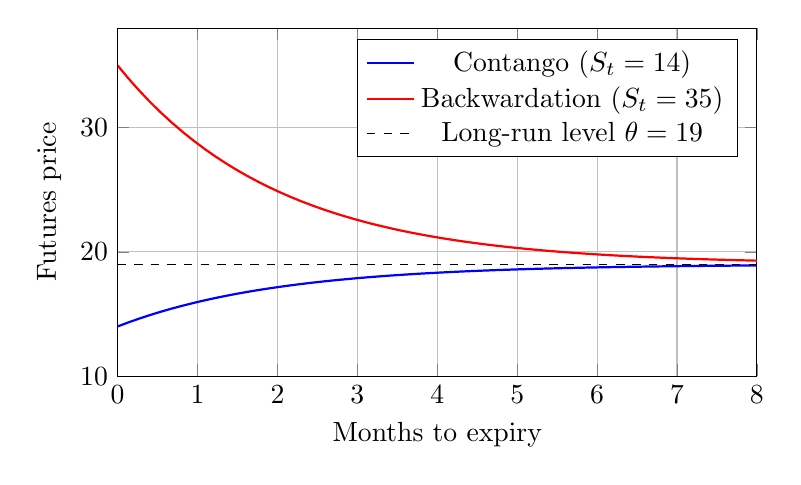
\begin{tikzpicture}
    \begin{axis}[
      width=0.8\linewidth, height=6cm,
      xlabel={Months to expiry}, ylabel={Futures price},
      xmin=0, xmax=8, ymin=10, ymax=38,
      legend pos=north east, grid=major
    ]
      \addplot[thick, blue, domain=0:8, samples=60] {19 + (14-19)*exp(-0.5*x)};
      \addlegendentry{Contango ($S_t=14$)}
      \addplot[thick, red, domain=0:8, samples=60] {19 + (35-19)*exp(-0.5*x)};
      \addlegendentry{Backwardation ($S_t=35$)}
      \addplot[dashed, black, domain=0:8] {19};
      \addlegendentry{Long-run level $\theta=19$}
    \end{axis}
  \end{tikzpicture}
  \caption{Stylized VIX futures curves from~\eqref{eq:stylized-curve} with assumed $\theta=19$ and $\kappa=0.5$ per month. Illustrative only, not market data.}
  \label{fig:term-structure}
\end{figure}

\begin{figure}[htbp]
  \centering
  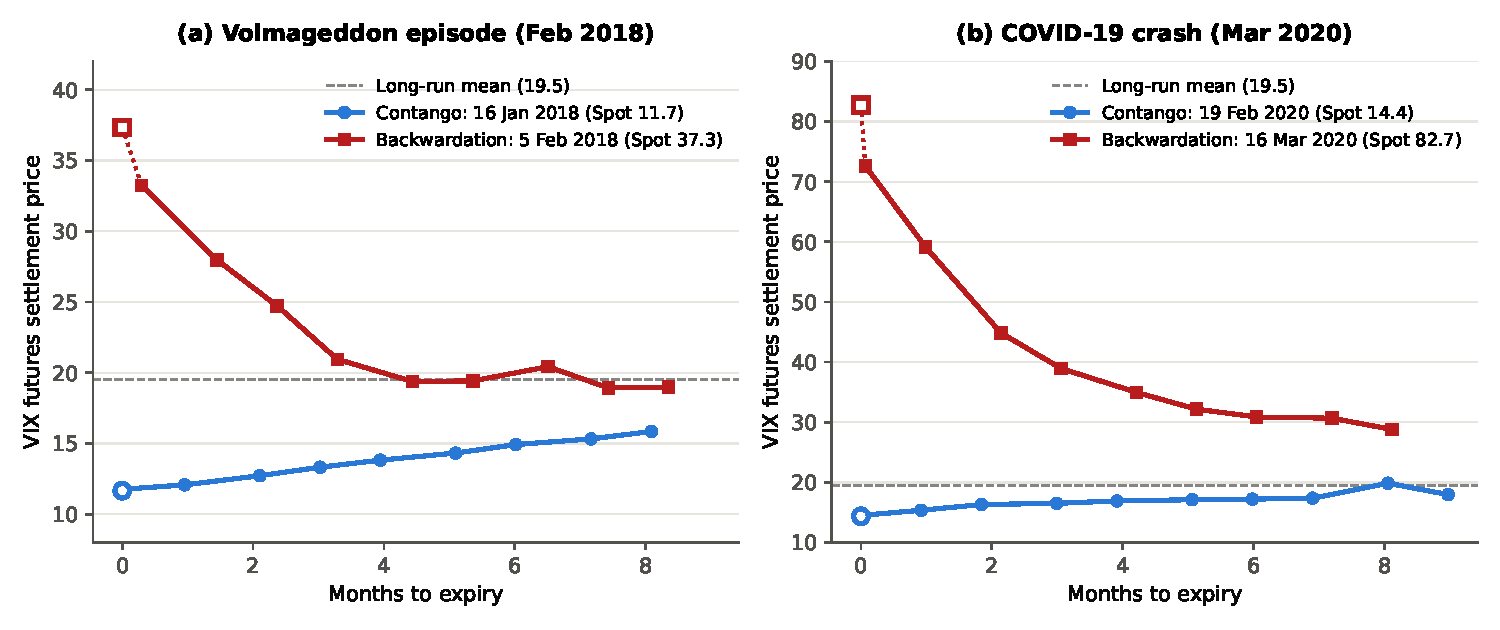
\includegraphics[width=\linewidth]{figures/vix_term_structure.pdf}
  \caption{Observed VIX futures term structure during calm and stressed markets: (a) the February 2018 Volmageddon episode (16 January vs.\ 5 February 2018) and (b) the COVID-19 market crash (19 February vs.\ 16 March 2020). Hollow markers at month 0 denote the prevailing spot VIX; solid markers denote official Cboe futures settlement prices. The dashed line marks the empirical long-run mean ($\approx 19.5$). Data: Cboe Futures Exchange and Cboe.}
  \label{fig:term-structure-real}
\end{figure}

\paragraph{Consequences for investors.} The shape of the curve determines the carry of a long or short volatility position. Summarizing the roll discussion in the previous section (see~\eqref{eq:roll}):

\begin{table}[htbp]
\centering
\small
\begin{tabular}{@{}lccc@{}}
\toprule
\textbf{Curve shape} & \textbf{Typical state} & \textbf{Long futures (roll)} & \textbf{Short futures (roll)}\\
\midrule
Contango & Calm market & Negative roll yield & Positive roll yield\\
Backwardation & Market stress & Positive roll yield & Negative roll yield\\
\bottomrule
\end{tabular}
\caption{Effect of term-structure shape on the carry of VIX futures positions, assuming an unchanged spot VIX.}
\label{tab:roll-summary}
\end{table}

A common summary of the slope is the \emph{basis} $F(t,T_1)-\text{VIX}_t$ or the relative spread $\big(F(t,T_2)-F(t,T_1)\big)/F(t,T_1)$ between the first two futures. These quantities will be used in the backtest to explain when a long-futures hedge is expensive to hold.
%
% Requires in the preamble: amsmath, booktabs, tikz, pgfplots
% (\pgfplotsset{compat=1.16}), and the macros \VIX, \verify, \figplaceholder.
% Uses labels from the discussion section: eq:vix-term, eq:vix-interp, eq:roll.
% New bibliography keys to add: cboewp (already used), cboevxfut, cboevxopt.
% =====================================================================



%=====================================================================
\subsection{Cboe VIX Methodology}
\label{sec:vix-method}
%=====================================================================

The VIX is a model-free estimate of the market's expected 30-day variance, computed from a \emph{strip} of out-of-the-money S\&P~500 (SPX) options. The calculation was introduced in Section~1.1.1: per-expiration variances are given by~\eqref{eq:vix-term} and combined by constant-maturity interpolation in~\eqref{eq:vix-interp}. Here we summarize the rules that determine \emph{which} options enter the calculation, since these rules matter for any implementation.

\paragraph{Options used.} The index uses both standard monthly SPX options (which expire on the third Friday of each month) and weekly SPX options (which expire on other Fridays) \cite{cboewp}. Combining monthly and weekly options ensures that there are always expirations bracketing the 30-day target. Only expirations with 23 to 37 days remaining are eligible: the two maturities immediately surrounding 30 days are designated as the near-term ($T_1$) and next-term ($T_2$) terms. Cboe calculates and disseminates the spot VIX every 15 seconds during trading hours using prevailing market quotes \cite{cboewp}.

\paragraph{Quotes and strike selection.} For each expiration the algorithm proceeds as follows:
\begin{enumerate}
  \item Find the forward level $F$ from put--call parity at the strike where the call and put mid-quotes are closest, and set $K_0$ to the strike at or immediately below $F$ (see Section~1.1.1).
  \item Starting at $K_0$ and moving to \emph{lower} strikes, select out-of-the-money puts. Starting at $K_0$ and moving to \emph{higher} strikes, select out-of-the-money calls. At $K_0$ itself the average of the call and put mid-quotes is used.
  \item Use the mid-quote $Q(K_i)=\tfrac12(\text{bid}+\text{ask})$ for each selected option. Options with a zero bid are never included.
  \item Stop moving outward in a given direction once two consecutive strikes with a zero bid are encountered. No strikes beyond that point are used, even if they have non-zero bids.
\end{enumerate}
The last rule truncates the strip in the far wings, where quotes are stale or non-informative and where a literal evaluation of the formula would be dominated by noise.

\paragraph{Why out-of-the-money options with $1/K^2$ weights.} Each selected option enters~\eqref{eq:vix-term} with weight proportional to $\Delta K_i/K_i^2$. Low-strike puts therefore receive more weight per unit of price than high-strike calls, because they insure against the large downside moves that contribute most to variance. This weighting is exactly the static-replication result for a variance swap, which is derived in the pricing section. Figure~\ref{fig:weights} illustrates the weight function.

\begin{figure}[htbp]
  \centering
  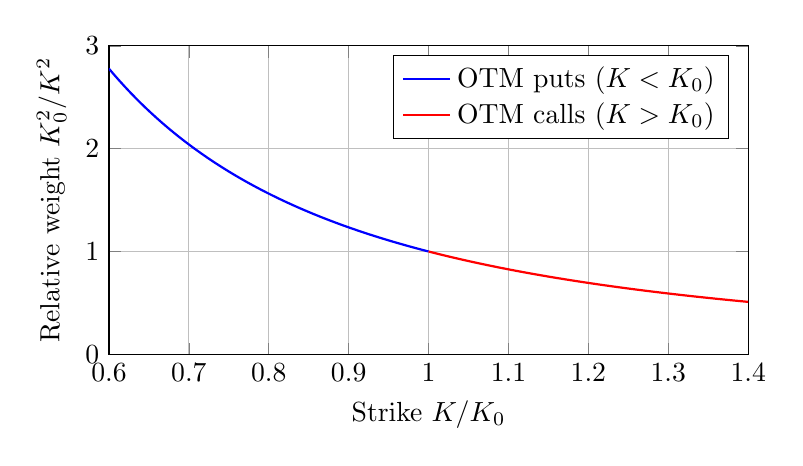
\begin{tikzpicture}
    \begin{axis}[
      width=0.8\linewidth, height=5.5cm,
      xlabel={Strike $K/K_0$}, ylabel={Relative weight $K_0^2/K^2$},
      xmin=0.6, xmax=1.4, ymin=0, ymax=3,
      legend pos=north east, grid=major
    ]
      \addplot[thick, blue, domain=0.6:1, samples=60] {1/x^2};
      \addlegendentry{OTM puts ($K<K_0$)}
      \addplot[thick, red, domain=1:1.4, samples=60] {1/x^2};
      \addlegendentry{OTM calls ($K>K_0$)}
    \end{axis}
  \end{tikzpicture}
  \caption{Variance-swap weight $\propto 1/K^2$ across the option strip (with $\Delta K$ held constant and normalized by $K_0$). Illustrative.}
  \label{fig:weights}
\end{figure}

\paragraph{Spot VIX versus the SOQ.} During trading hours, the spot VIX reflects the average of bid and ask quotes and interpolates between two maturities using~\eqref{eq:vix-interp}. In contrast, expiring VIX futures and options settle for cash against a single official benchmark called the \emph{Special Opening Quotation} (SOQ) \cite{cboewp}. The SOQ differs from the spot VIX in two important ways:
\begin{enumerate}
  \item \textbf{Single 30-day expiration.} Because settlement occurs on a Wednesday morning exactly 30 days before the underlying SPX options expire, the SOQ evaluates the forward variance formula~\eqref{eq:vix-term} on that single expiration. No two-maturity interpolation~\eqref{eq:vix-interp} is needed.
  \item \textbf{Actual opening trade prices.} Rather than midpoint quotes, the SOQ uses actual executed prices from a special opening auction on settlement morning (falling back to mid-quotes only if an option does not trade).
\end{enumerate}
Because of these structural differences, the settlement SOQ can diverge from the spot VIX displayed on screens that morning.

%=====================================================================
\subsection{VIX Futures}
\label{sec:vix-futures}
%=====================================================================

A VIX future is a cash-settled contract whose final value is the VIX SOQ on the expiration date \cite{cboevxfut}. The contract is not on the VIX ``spot'' that traders see during the day, nor on a basket of SPX options held by the exchange; it is a standardized bet on the SOQ.

\paragraph{Key contract terms.}
\begin{table}[htbp]
\centering
\small
\begin{tabular}{@{}p{3.6cm}p{11cm}@{}}
\toprule
\textbf{Term} & \textbf{Specification}\\
\midrule
Underlying & Cboe Volatility Index (settled at the SOQ)\\
Multiplier & \$1{,}000 per index point\\
Settlement & Cash, at the SOQ on the final settlement date\\
Final settlement date & Wednesday that is 30 days before the third Friday of the following calendar month (previous business day if a holiday)\verify\\
Expirations & Several consecutive monthly expirations, plus weekly series\verify\\
\bottomrule
\end{tabular}
\caption{Principal terms of standard VIX futures. Check the exchange contract specification before finalizing.}
\label{tab:vx-spec}
\end{table}

The settlement date is chosen so that the 30-day window of the SPX options used to compute the SOQ begins at the futures expiration. The futures are therefore a view on volatility over the \emph{next} 30 days \emph{starting at expiry}, not over the life of the contract.

\paragraph{Payoff.} Entering a long position at futures price $F_0$ and holding until expiration $T$ produces the profit
\begin{equation}
  \text{P\&L} = 1{,}000\times(\text{SOQ}_T - F_0),
\end{equation}
before margin and financing considerations. For example, buying at $F_0=18.50$ and settling at $\text{SOQ}_T = 21.30$ gives $1{,}000\times 2.80=\$2{,}800$ per contract (hypothetical numbers).

\paragraph{Futures versus spot VIX.} Before expiry the futures price is not equal to the spot VIX. Under the risk-neutral measure $\mathbb{Q}$,
\begin{equation}
  F(t,T) = \mathbb{E}^{\mathbb{Q}}\!\left[\text{SOQ}_T \,\middle|\, \mathcal{F}_t\right],
  \label{eq:fut-expect}
\end{equation}
so the futures price is the expected \emph{future} level of the index. It differs from the spot VIX because (i) the market expects mean reversion in volatility, (ii) the VIX is the square root of a variance, introducing a convexity effect (Jensen's inequality), and (iii) hedgers pay a premium for volatility protection. The convexity effect is quantified in the pricing and simulation sections.

\paragraph{Smaller contracts.} Cboe also lists mini VIX futures with a smaller multiplier (\$100 per point)\verify, useful for smaller accounts and hedges.

%=====================================================================
\subsection{VIX Options}
\label{sec:vix-options}
%=====================================================================

VIX options are European-style, cash-settled options on the VIX with a multiplier of \$100 per index point \cite{cboevxopt}. They settle to the same SOQ as the futures with the matching expiration.

\begin{table}[htbp]
\centering
\small
\begin{tabular}{@{}p{3.6cm}p{11cm}@{}}
\toprule
\textbf{Term} & \textbf{Specification}\\
\midrule
Underlying & VIX (settled at the SOQ); priced off the VIX future with the same expiration\\
Style & European\\
Multiplier & \$100 per index point\\
Settlement & Cash, at the SOQ on the expiration date\\
Expirations & Same schedule as VIX futures (monthly, with weekly series)\verify\\
\bottomrule
\end{tabular}
\caption{Principal terms of VIX options.}
\label{tab:vix-options}
\end{table}

\paragraph{Payoff.} At expiration a call with strike $K$ pays $100\times\max(\text{SOQ}_T-K,\,0)$ and a put pays $100\times\max(K-\text{SOQ}_T,\,0)$. For instance, a call with $K=20$ settling at $\text{SOQ}_T=23.50$ pays $100\times 3.50 = \$350$ (hypothetical).

\paragraph{The underlying is the future, not spot.} Because the VIX itself is not tradable, VIX options cannot be hedged with the spot index. Their effective underlying is the VIX future with the same expiration, which \emph{can} be traded. Consequently put--call parity takes the form
\begin{equation}
  C(K,T) - P(K,T) = e^{-r(T-t)}\big(F(t,T)-K\big),
  \label{eq:vix-pcp}
\end{equation}
where $F(t,T)$ is the VIX future for the same expiration, \emph{not} the spot VIX. Pricing VIX options therefore requires a model of the dynamics of $F(t,T)$, usually a stochastic-volatility model; this is the role of the Heston simulation later in this report.

%=====================================================================
\subsection{The Term Structure of VIX Futures}
\label{sec:term-structure}
%=====================================================================

At each date $t$ there is a family of listed VIX futures with different expirations. The map $T\mapsto F(t,T)$ is the \emph{term structure} (or \emph{forward curve}) of volatility.

\begin{itemize}
  \item \textbf{Contango:} the curve slopes upward, $F(t,T_1) < F(t,T_2) < \cdots$, with the front future typically above the spot VIX. This is the usual shape in calm markets.
  \item \textbf{Backwardation:} the curve slopes downward, $F(t,T_1) > F(t,T_2) > \cdots$, with the spot VIX at or above the front future. This typically occurs during market stress, when the spot VIX spikes.
\end{itemize}

\paragraph{Why the curve has these shapes.} The VIX is mean-reverting: it tends to return toward a long-run level $\theta$. A stylized representation, ignoring convexity and risk premia, is
\begin{equation}
  F(t,T) \approx \theta + (S_t-\theta)\,e^{-\kappa(T-t)},
  \label{eq:stylized-curve}
\end{equation}
where $S_t$ is the current spot VIX and $\kappa>0$ is the speed of mean reversion. When $S_t<\theta$ (calm markets) the curve rises toward $\theta$ (contango); when $S_t>\theta$ (stressed markets) it falls toward $\theta$ (backwardation). Figure~\ref{fig:term-structure} illustrates both cases schematically, and Figure~\ref{fig:term-structure-real} displays the actual observed term structures during the February 2018 Volmageddon and March 2020 COVID-19 episodes. In practice, a risk premium paid by hedgers also pushes the curve upward, which is one reason contango is more common than backwardation\verify.

\begin{figure}[htbp]
  \centering
  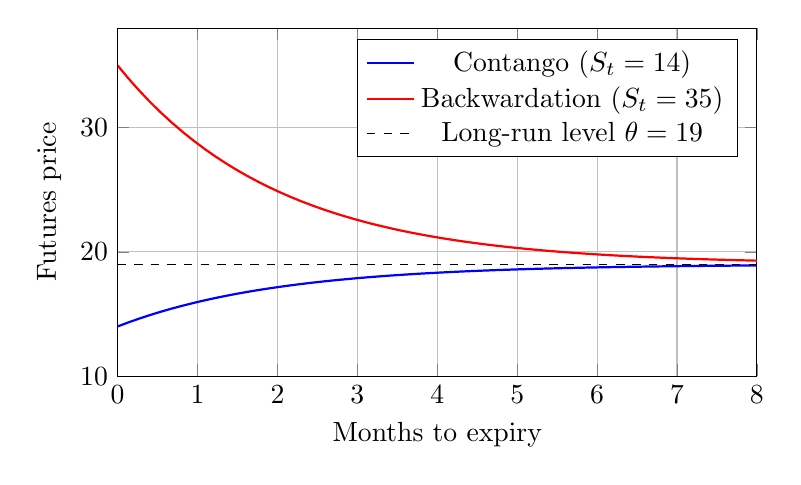
\begin{tikzpicture}
    \begin{axis}[
      width=0.8\linewidth, height=6cm,
      xlabel={Months to expiry}, ylabel={Futures price},
      xmin=0, xmax=8, ymin=10, ymax=38,
      legend pos=north east, grid=major
    ]
      \addplot[thick, blue, domain=0:8, samples=60] {19 + (14-19)*exp(-0.5*x)};
      \addlegendentry{Contango ($S_t=14$)}
      \addplot[thick, red, domain=0:8, samples=60] {19 + (35-19)*exp(-0.5*x)};
      \addlegendentry{Backwardation ($S_t=35$)}
      \addplot[dashed, black, domain=0:8] {19};
      \addlegendentry{Long-run level $\theta=19$}
    \end{axis}
  \end{tikzpicture}
  \caption{Stylized VIX futures curves from~\eqref{eq:stylized-curve} with assumed $\theta=19$ and $\kappa=0.5$ per month. Illustrative only, not market data.}
  \label{fig:term-structure}
\end{figure}

\begin{figure}[htbp]
  \centering
  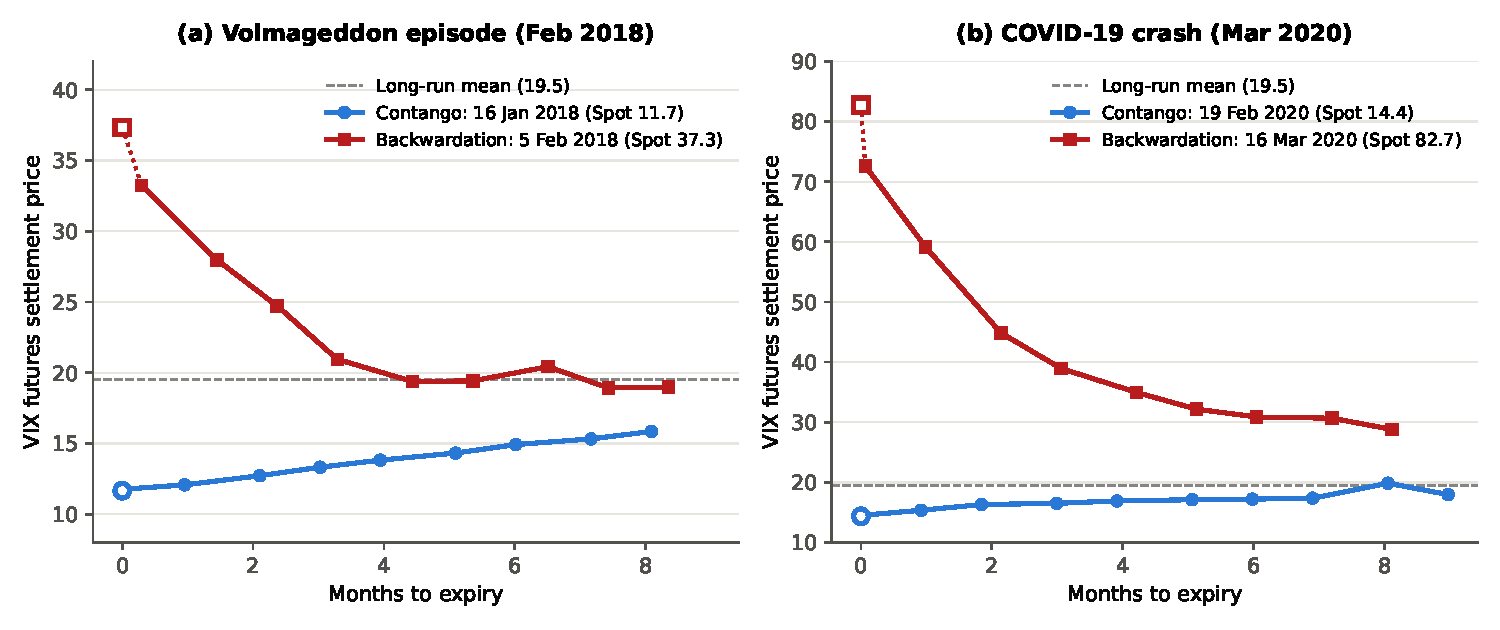
\includegraphics[width=\linewidth]{figures/vix_term_structure.pdf}
  \caption{Observed VIX futures term structure during calm and stressed markets: (a) the February 2018 Volmageddon episode (16 January vs.\ 5 February 2018) and (b) the COVID-19 market crash (19 February vs.\ 16 March 2020). Hollow markers at month 0 denote the prevailing spot VIX; solid markers denote official Cboe futures settlement prices. The dashed line marks the empirical long-run mean ($\approx 19.5$). Data: Cboe Futures Exchange and Cboe.}
  \label{fig:term-structure-real}
\end{figure}

\paragraph{Consequences for investors.} The shape of the curve determines the carry of a long or short volatility position. Summarizing the roll discussion in the previous section (see~\eqref{eq:roll}):

\begin{table}[htbp]
\centering
\small
\begin{tabular}{@{}lccc@{}}
\toprule
\textbf{Curve shape} & \textbf{Typical state} & \textbf{Long futures (roll)} & \textbf{Short futures (roll)}\\
\midrule
Contango & Calm market & Negative roll yield & Positive roll yield\\
Backwardation & Market stress & Positive roll yield & Negative roll yield\\
\bottomrule
\end{tabular}
\caption{Effect of term-structure shape on the carry of VIX futures positions, assuming an unchanged spot VIX.}
\label{tab:roll-summary}
\end{table}

A common summary of the slope is the \emph{basis} $F(t,T_1)-\text{VIX}_t$ or the relative spread $\big(F(t,T_2)-F(t,T_1)\big)/F(t,T_1)$ between the first two futures. These quantities will be used in the backtest to explain when a long-futures hedge is expensive to hold.